% Generated by Sphinx.
\def\sphinxdocclass{report}
\documentclass[letterpaper,10pt,english]{sphinxmanual}
\usepackage[utf8]{inputenc}
\DeclareUnicodeCharacter{00A0}{\nobreakspace}
\usepackage[T1]{fontenc}
\usepackage{babel}
\usepackage{times}
\usepackage[Bjarne]{fncychap}
\usepackage{longtable}
\usepackage{sphinx}
\usepackage{multirow}


\title{Create Image Galleries and Slide Shows Documentation}
\date{December 22, 2011}
\release{0}
\author{Melissa Anderson}
\newcommand{\sphinxlogo}{}
\renewcommand{\releasename}{Release}
\makeindex

\makeatletter
\def\PYG@reset{\let\PYG@it=\relax \let\PYG@bf=\relax%
    \let\PYG@ul=\relax \let\PYG@tc=\relax%
    \let\PYG@bc=\relax \let\PYG@ff=\relax}
\def\PYG@tok#1{\csname PYG@tok@#1\endcsname}
\def\PYG@toks#1+{\ifx\relax#1\empty\else%
    \PYG@tok{#1}\expandafter\PYG@toks\fi}
\def\PYG@do#1{\PYG@bc{\PYG@tc{\PYG@ul{%
    \PYG@it{\PYG@bf{\PYG@ff{#1}}}}}}}
\def\PYG#1#2{\PYG@reset\PYG@toks#1+\relax+\PYG@do{#2}}

\def\PYG@tok@gd{\def\PYG@tc##1{\textcolor[rgb]{0.63,0.00,0.00}{##1}}}
\def\PYG@tok@gu{\let\PYG@bf=\textbf\def\PYG@tc##1{\textcolor[rgb]{0.50,0.00,0.50}{##1}}}
\def\PYG@tok@gt{\def\PYG@tc##1{\textcolor[rgb]{0.00,0.25,0.82}{##1}}}
\def\PYG@tok@gs{\let\PYG@bf=\textbf}
\def\PYG@tok@gr{\def\PYG@tc##1{\textcolor[rgb]{1.00,0.00,0.00}{##1}}}
\def\PYG@tok@cm{\let\PYG@it=\textit\def\PYG@tc##1{\textcolor[rgb]{0.25,0.50,0.56}{##1}}}
\def\PYG@tok@vg{\def\PYG@tc##1{\textcolor[rgb]{0.73,0.38,0.84}{##1}}}
\def\PYG@tok@m{\def\PYG@tc##1{\textcolor[rgb]{0.13,0.50,0.31}{##1}}}
\def\PYG@tok@mh{\def\PYG@tc##1{\textcolor[rgb]{0.13,0.50,0.31}{##1}}}
\def\PYG@tok@cs{\def\PYG@tc##1{\textcolor[rgb]{0.25,0.50,0.56}{##1}}\def\PYG@bc##1{\colorbox[rgb]{1.00,0.94,0.94}{##1}}}
\def\PYG@tok@ge{\let\PYG@it=\textit}
\def\PYG@tok@vc{\def\PYG@tc##1{\textcolor[rgb]{0.73,0.38,0.84}{##1}}}
\def\PYG@tok@il{\def\PYG@tc##1{\textcolor[rgb]{0.13,0.50,0.31}{##1}}}
\def\PYG@tok@go{\def\PYG@tc##1{\textcolor[rgb]{0.19,0.19,0.19}{##1}}}
\def\PYG@tok@cp{\def\PYG@tc##1{\textcolor[rgb]{0.00,0.44,0.13}{##1}}}
\def\PYG@tok@gi{\def\PYG@tc##1{\textcolor[rgb]{0.00,0.63,0.00}{##1}}}
\def\PYG@tok@gh{\let\PYG@bf=\textbf\def\PYG@tc##1{\textcolor[rgb]{0.00,0.00,0.50}{##1}}}
\def\PYG@tok@ni{\let\PYG@bf=\textbf\def\PYG@tc##1{\textcolor[rgb]{0.84,0.33,0.22}{##1}}}
\def\PYG@tok@nl{\let\PYG@bf=\textbf\def\PYG@tc##1{\textcolor[rgb]{0.00,0.13,0.44}{##1}}}
\def\PYG@tok@nn{\let\PYG@bf=\textbf\def\PYG@tc##1{\textcolor[rgb]{0.05,0.52,0.71}{##1}}}
\def\PYG@tok@no{\def\PYG@tc##1{\textcolor[rgb]{0.38,0.68,0.84}{##1}}}
\def\PYG@tok@na{\def\PYG@tc##1{\textcolor[rgb]{0.25,0.44,0.63}{##1}}}
\def\PYG@tok@nb{\def\PYG@tc##1{\textcolor[rgb]{0.00,0.44,0.13}{##1}}}
\def\PYG@tok@nc{\let\PYG@bf=\textbf\def\PYG@tc##1{\textcolor[rgb]{0.05,0.52,0.71}{##1}}}
\def\PYG@tok@nd{\let\PYG@bf=\textbf\def\PYG@tc##1{\textcolor[rgb]{0.33,0.33,0.33}{##1}}}
\def\PYG@tok@ne{\def\PYG@tc##1{\textcolor[rgb]{0.00,0.44,0.13}{##1}}}
\def\PYG@tok@nf{\def\PYG@tc##1{\textcolor[rgb]{0.02,0.16,0.49}{##1}}}
\def\PYG@tok@si{\let\PYG@it=\textit\def\PYG@tc##1{\textcolor[rgb]{0.44,0.63,0.82}{##1}}}
\def\PYG@tok@s2{\def\PYG@tc##1{\textcolor[rgb]{0.25,0.44,0.63}{##1}}}
\def\PYG@tok@vi{\def\PYG@tc##1{\textcolor[rgb]{0.73,0.38,0.84}{##1}}}
\def\PYG@tok@nt{\let\PYG@bf=\textbf\def\PYG@tc##1{\textcolor[rgb]{0.02,0.16,0.45}{##1}}}
\def\PYG@tok@nv{\def\PYG@tc##1{\textcolor[rgb]{0.73,0.38,0.84}{##1}}}
\def\PYG@tok@s1{\def\PYG@tc##1{\textcolor[rgb]{0.25,0.44,0.63}{##1}}}
\def\PYG@tok@gp{\let\PYG@bf=\textbf\def\PYG@tc##1{\textcolor[rgb]{0.78,0.36,0.04}{##1}}}
\def\PYG@tok@sh{\def\PYG@tc##1{\textcolor[rgb]{0.25,0.44,0.63}{##1}}}
\def\PYG@tok@ow{\let\PYG@bf=\textbf\def\PYG@tc##1{\textcolor[rgb]{0.00,0.44,0.13}{##1}}}
\def\PYG@tok@sx{\def\PYG@tc##1{\textcolor[rgb]{0.78,0.36,0.04}{##1}}}
\def\PYG@tok@bp{\def\PYG@tc##1{\textcolor[rgb]{0.00,0.44,0.13}{##1}}}
\def\PYG@tok@c1{\let\PYG@it=\textit\def\PYG@tc##1{\textcolor[rgb]{0.25,0.50,0.56}{##1}}}
\def\PYG@tok@kc{\let\PYG@bf=\textbf\def\PYG@tc##1{\textcolor[rgb]{0.00,0.44,0.13}{##1}}}
\def\PYG@tok@c{\let\PYG@it=\textit\def\PYG@tc##1{\textcolor[rgb]{0.25,0.50,0.56}{##1}}}
\def\PYG@tok@mf{\def\PYG@tc##1{\textcolor[rgb]{0.13,0.50,0.31}{##1}}}
\def\PYG@tok@err{\def\PYG@bc##1{\fcolorbox[rgb]{1.00,0.00,0.00}{1,1,1}{##1}}}
\def\PYG@tok@kd{\let\PYG@bf=\textbf\def\PYG@tc##1{\textcolor[rgb]{0.00,0.44,0.13}{##1}}}
\def\PYG@tok@ss{\def\PYG@tc##1{\textcolor[rgb]{0.32,0.47,0.09}{##1}}}
\def\PYG@tok@sr{\def\PYG@tc##1{\textcolor[rgb]{0.14,0.33,0.53}{##1}}}
\def\PYG@tok@mo{\def\PYG@tc##1{\textcolor[rgb]{0.13,0.50,0.31}{##1}}}
\def\PYG@tok@mi{\def\PYG@tc##1{\textcolor[rgb]{0.13,0.50,0.31}{##1}}}
\def\PYG@tok@kn{\let\PYG@bf=\textbf\def\PYG@tc##1{\textcolor[rgb]{0.00,0.44,0.13}{##1}}}
\def\PYG@tok@o{\def\PYG@tc##1{\textcolor[rgb]{0.40,0.40,0.40}{##1}}}
\def\PYG@tok@kr{\let\PYG@bf=\textbf\def\PYG@tc##1{\textcolor[rgb]{0.00,0.44,0.13}{##1}}}
\def\PYG@tok@s{\def\PYG@tc##1{\textcolor[rgb]{0.25,0.44,0.63}{##1}}}
\def\PYG@tok@kp{\def\PYG@tc##1{\textcolor[rgb]{0.00,0.44,0.13}{##1}}}
\def\PYG@tok@w{\def\PYG@tc##1{\textcolor[rgb]{0.73,0.73,0.73}{##1}}}
\def\PYG@tok@kt{\def\PYG@tc##1{\textcolor[rgb]{0.56,0.13,0.00}{##1}}}
\def\PYG@tok@sc{\def\PYG@tc##1{\textcolor[rgb]{0.25,0.44,0.63}{##1}}}
\def\PYG@tok@sb{\def\PYG@tc##1{\textcolor[rgb]{0.25,0.44,0.63}{##1}}}
\def\PYG@tok@k{\let\PYG@bf=\textbf\def\PYG@tc##1{\textcolor[rgb]{0.00,0.44,0.13}{##1}}}
\def\PYG@tok@se{\let\PYG@bf=\textbf\def\PYG@tc##1{\textcolor[rgb]{0.25,0.44,0.63}{##1}}}
\def\PYG@tok@sd{\let\PYG@it=\textit\def\PYG@tc##1{\textcolor[rgb]{0.25,0.44,0.63}{##1}}}

\def\PYGZbs{\char`\\}
\def\PYGZus{\char`\_}
\def\PYGZob{\char`\{}
\def\PYGZcb{\char`\}}
\def\PYGZca{\char`\^}
\def\PYGZsh{\char`\#}
\def\PYGZpc{\char`\%}
\def\PYGZdl{\char`\$}
\def\PYGZti{\char`\~}
% for compatibility with earlier versions
\def\PYGZat{@}
\def\PYGZlb{[}
\def\PYGZrb{]}
\makeatother

\begin{document}

\maketitle
\tableofcontents
\phantomsection\label{index::doc}


Contents:


\chapter{Build Image Galleries and Slideshows}
\label{recipe:build-image-galleries-and-slideshows}\label{recipe:welcome-to-create-image-galleries-and-slide-shows-s-documentation}\label{recipe::doc}

\section{Staple}
\label{recipe:staple}\begin{enumerate}
\item {} 
\href{http://drupal.org/project/ctools}{http://drupal.org/project/ctools} - Enable Chaos Tools (all others are not needed)

\item {} 
\href{http://drupal.org/project/views}{http://drupal.org/project/views} - Enable Views and Views UI

\item {} 
\href{http://drupal.org/project/libraries}{http://drupal.org/project/libraries} - Enable Libraries

\item {} 
\href{http://drupal.org/project/views\_slideshow}{http://drupal.org/project/views\_slideshow} - Enable Views Slideshow

\end{enumerate}
\begin{description}
\item[{\textbf{Drush users:}}] \leavevmode
\begin{DUlineblock}{0em}
\item[] drush dl ctools views libraries views\_slideshow
\item[] drush en ctools views views\_ui libraries views\_slideshow -y
\end{DUlineblock}

\end{description}


\section{Speciality}
\label{recipe:speciality}
Views Slideshow module uses two external libraries.

Required for basic slide show functionality:
\begin{enumerate}
\item {} 
Visit \href{http://malsup.com/jquery/cycle/download.html}{http://malsup.com/jquery/cycle/download.html}

\item {} 
Right-click the link to “Cycle Plugin”

\item {} 
Save the link into sites/all/libraries/jquery.cycle so that the final path looks like sites/all/libraries/jquery.cycle/jquery.cycle.all.js

\end{enumerate}

Recommended for advanced features:
\begin{enumerate}
\item {} 
Visit \href{https://github.com/douglascrockford/JSON-js/downloads}{https://github.com/douglascrockford/JSON-js/downloads} and download the appropriate format, .zip or .tar.gz, for your environment.

\item {} 
Extract to sites/all/libraries

\item {} 
Rename the directory (which begins with douglascrockford-) to json2 so that the final path looks like: sites/all/libraries/json2/json2.js

\end{enumerate}


\section{Part 1: Build the form for creating galleries}
\label{recipe:part-1-build-the-form-for-creating-galleries}

\subsection{Step 1.1: Add a new content type called Gallery}
\label{recipe:step-1-1-add-a-new-content-type-called-gallery}
\emph{Structure \textgreater{} Content types \textgreater{} +Add new content type}

Name: Gallery

Description: Create an image gallery with slide show controls.

\begin{tabulary}{\linewidth}{|L|L|}
\hline

Submission Form Settings
 & 
Title field label: Gallery name
\\\hline

Publishing Options
 & 
{[}√{]} Published (Check only this option; uncheck others)
\\\hline

Display Settings
 & 
{[}  {]} Display author and date information (Uncheck this)
\\\hline

Comment Settings
 & 
Closed (Select Closed)
\\\hline

Menu Settings
 & 
{[}  {]} Uncheck all menus
\\\hline
\end{tabulary}



\subsection{Step 1.2: Add an image field}
\label{recipe:step-1-2-add-an-image-field}
\emph{Structure \textgreater{} Content types \textgreater{} Gallery \textgreater{} Manage fields}


\subsubsection{Add new field}
\label{recipe:add-new-field}\begin{enumerate}
\item {} 
Label: Gallery Image

\item {} 
Field name: gallery\_image

\item {} 
Type of data to store: Image

\item {} 
Form element to edit the data: Image

\end{enumerate}


\subsubsection{Field Settings}
\label{recipe:field-settings}
Leave as is. Public files selected, no default image


\subsubsection{GALLERY Settings}
\label{recipe:gallery-settings}
There are a lot of settings here! Accept the defaults EXCEPT the following:

File directory: gallery

Minimum image resolution: 480 x 360

We’ll be displaying Drupal’s pre-fomatted Large image size of 480 x 360. By requiring images to be at least that large here, we can prevent jarring changes in size and eliminate white space between main images and thumbnails.

{[}√{]} Enable Title field


\subsubsection{GALLERY IMAGE Field Settings}
\label{recipe:gallery-image-field-settings}
Number of values: 10


\subsection{Step 1.3: Create proper paths}
\label{recipe:step-1-3-create-proper-paths}
\emph{Configuration \textgreater{} Search and Metadata: URL aliases \textgreater{} Patterns}

Later on, we’ll be creating a landing page at /galleries, so we’re adding that to the path now.

Pattern for all Gallery paths: galleries/{[}node:title{]}


\subsection{Step 1.4: Create a test gallery}
\label{recipe:step-1-4-create-a-test-gallery}
\emph{Content \textgreater{} Add content \textgreater{} Gallery}
\begin{enumerate}
\item {} 
Gallery name: Test Gallery

\item {} 
Body text: Optional

\item {} 
Browse and upload at least 4 images, giving each one a title.

\item {} 
Check the URL pattern is what you expect, something like: \href{http://tests.l/galleries/test-gallery}{http://tests.l/galleries/test-gallery}

\end{enumerate}


\subsection{Step 1.5: Hide the default display of images}
\label{recipe:step-1-5-hide-the-default-display-of-images}
\emph{Structure \textgreater{} Content types \textgreater{} Gallery \textgreater{} Manage display}
\begin{enumerate}
\item {} 
Set the Default display setting format for Image to Hidden.

\item {} 
Verify the Teaser display format is hidden. It should already be set that way.

\item {} 
Go to Content and view the gallery you created in step 1.4

\item {} 
You should see nothing but body text you entered.

\end{enumerate}


\section{Step 2: Create custom image sizes}
\label{recipe:step-2-create-custom-image-sizes}

\subsection{Gallery thumbnails}
\label{recipe:gallery-thumbnails}
\emph{Configuration \textgreater{} Media \textgreater{} Image styles \textgreater{} +Add style}

The thumbnail settings are chosen so the images stay mostly proportional to an 800 x 600 original and so five thumbnails fit width-wise under the 480 x 360 Large image style that comes with Drupal by default.
\begin{enumerate}
\item {} 
Image style name: gallery\_thumb

\item {} 
In Effect, choose Scale and crop, then click Add

\item {} 
Width: 90

\item {} 
Height: 70

\item {} 
Click the Add effect button (Your changes are saved; the button on the next page is just for reordering the effects)

\end{enumerate}


\subsection{Index thumbnails}
\label{recipe:index-thumbnails}
\emph{Configuration \textgreater{} Media \textgreater{} Image styles \textgreater{} +Add style}

Add a second style for the index of galleries on the site.
\begin{enumerate}
\item {} 
Click +Add style again

\item {} 
Image style name: gallery\_index

\item {} 
In Effect, choose Scale and crop, then click Add

\item {} 
Width: 180

\item {} 
Height: 140

\item {} 
Click the Add effect button (Your changes are saved; the button on the next page is just for reordering the effects)

\end{enumerate}


\section{Step 3: Create the galleries}
\label{recipe:step-3-create-the-galleries}
Views delivers extraordinary power to the non-programmer, and the price is a densely-packed interface. We describe the steps below, but there's a place where the screen cast is worth a thousand words!


\subsection{3.1: Create the actual gallery display}
\label{recipe:create-the-actual-gallery-display}
\emph{Structure \textgreater{} Views \textgreater{} +Add new view}

On the introductory Views page:
\begin{figure}[htbp]
\centering

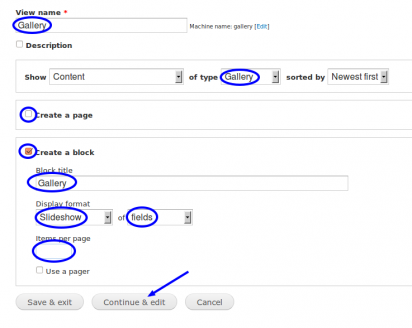
\includegraphics{slideshow-3.1-412x328.png}
{\small \begin{enumerate}
\item {} 
View name: Gallery

\item {} 
Show content of type Gallery sorted by Newest first

\item {} 
{[}  {]}   Uncheck Page

\item {} 
{[}√{]}  Check Block

\item {} 
Block title: Gallery

\item {} 
Display fomat: Slideshow of fields

\item {} 
Items per page: (Leave this blank)

\item {} 
Continue \& Edit

\item {} 
Save

\end{enumerate}
}\end{figure}
\begin{figure}[htbp]
\centering

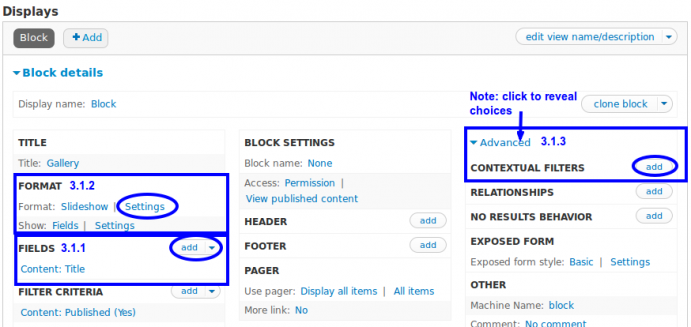
\includegraphics{slideshow-3.1-main.png}
{\small 
In main Views interface, we'll configure three areas:

\begin{DUlineblock}{0em}
\item[] 3.1.1 - available fields
\item[] 3.1.2 - row style settings,
\item[] 3.1.3 - the contextual filter.
\end{DUlineblock}

We’ll set them up in this order because they depend upon each other, even though they’re visually in a different order.
}\end{figure}


\subsubsection{3.1.1 Add Fields}
\label{recipe:add-fields}
First, add the main gallery image:
\begin{enumerate}
\item {} 
Fields: add

\item {} 
From the popup, select: Content: Gallery image

\item {} 
Appears in: node:gallery.

\item {} 
{[}  {]} Remove the check in the box Create a label

\item {} 
Set the Image style to large.

\item {} 
Multiple Field Values: Uncheck Display all values in the same row

\item {} 
Apply (All displays)

\end{enumerate}

Second, add the thumnail gallery images. Much like the first step:
\begin{enumerate}
\item {} 
Fields: add

\item {} 
From the popup, select: Content: Gallery image

\item {} 
Appears in: node:gallery.

\item {} 
{[}  {]} Remove the check in the box Create a label

\item {} 
{[}√{]} Check Exclude from display

\item {} 
Set the Image style to gallery\_thumb.

\item {} 
Multiple Field Values: Uncheck Display all values in the same row

\item {} 
Apply (All displays)

\end{enumerate}

Next, add the title.
\begin{enumerate}
\item {} 
Fileds: add

\item {} 
From the popup, select:Content: Gallery image

\item {} 
Appears in: node:gallery

\item {} 
{[}   Remove the check in the box Create a label

\item {} 
Leave other visible settings at their default

\item {} 
Multiple Field Values: Uncheck Display all values in the same row

\item {} 
Expand Rewrite Results

\item {} 
Rewrite the output of this field

\item {} 
In the text field, enter {[}field\_gallery\_image\_2-title{]} (View the available patterns by expanding Rep lacement patterns.)

\item {} 
Apply (all displays)

\end{enumerate}

You now have three fields, all named the same thing but configured differently, the main image, the thumbnails, and the image titles.

Finally, remove the Content Title since it's the name of the gallery (redundant) and not the name of the image.
\begin{enumerate}
\item {} 
Cllick the link Content: Title

\item {} 
Scroll and click Remove

\end{enumerate}


\subsubsection{3.1.2 Format}
\label{recipe:format}\begin{enumerate}
\item {} 
Format: Settings

\item {} 
In the Top Widgets section, check Controls.

\item {} 
In the Bottom Widgets section, check Pager and choose the middle instance of

\item {} 
Content: Gallery Image

\item {} 
Apply (All displays)

\end{enumerate}


\subsubsection{3.1.3 Advanced}
\label{recipe:advanced}\begin{enumerate}
\item {} 
Contextual Filter (Add)

\item {} 
Content: Nid

\item {} 
Choose Provide a default value \textgreater{} Type: Content ID from URL

\item {} 
Apply (All displays)

\end{enumerate}

Be sure to save the view!


\subsection{3.2: Place and configure the block}
\label{recipe:place-and-configure-the-block}
\emph{Structure \textgreater{} Blocks \textgreater{} Views: Galleries \textgreater{} Configure}

By configuring the block to display only on Gallery content types we prevent it from being called on a view, and by listing it only on specific pages we prevent it from appearing on the Edit tab.

Block title:  \textless{}none\textgreater{}
Region Settings
Custom (default theme)
Content
Visibility Settings

\begin{tabulary}{\linewidth}{|L|L|}
\hline

Pages
 & 
◉ Only the listed pages (Select this and enter the text below)
galleries*
\\\hline

Content types
 & 
{[}√{]} Gallery (Check only this option)
\\\hline

Roles
 & 
(Leave as is)
\\\hline

Users
 & 
(Leave as is)
\\\hline
\end{tabulary}



\section{Step 4: Create an index of all galleries}
\label{recipe:step-4-create-an-index-of-all-galleries}
\emph{Structure \textgreater{} Views \textgreater{} +Add new view}

You could create the gallery index page in the same view as the gallery block by adding a Page display, but the settings are different enough that they don’t gain a lot by sharing defaults, so we’ll create this as a separate view.


\subsection{4.1 Add a new view}
\label{recipe:add-a-new-view}

\subsubsection{Intro screen}
\label{recipe:intro-screen}\begin{enumerate}
\item {} 
View name: Galleries

\item {} 
Show Content of type Gallery sorted by Newest first

\item {} 
{[}√{]}  Create a page

\item {} 
Page title: Galleries

\item {} 
Display format: Grid of fields

\item {} 
{[}√{]}  Create a menu link

\item {} 
Menu: Main menu

\item {} 
Menu link title: Galleries

\item {} 
Save and continue

\end{enumerate}


\subsubsection{Fields}
\label{recipe:fields}
Add
\begin{enumerate}
\item {} 
Gallery image

\item {} 
{[}  {]}  Uncheck Create a label

\item {} 
Formatter: Image (no change)

\item {} 
Image style: medium

\item {} 
Link image to: Content

\item {} 
Apply (all displays)

\item {} 
Save

\end{enumerate}

Be sure to save the view!


\section{Part 5: Style the Gallery}
\label{recipe:part-5-style-the-gallery}

\subsection{5.1 Open custom.css}
\label{recipe:open-custom-css}
You can edit your style sheet any way that is comfortable for you. If you need more support than the username and password for your sandbox, see Connecting to your sandbox with sFTP at \href{http://training.opensourcery.com/basics/sftp}{http://training.opensourcery.com/basics/sftp}


\subsection{5.2 Add gallery styling}
\label{recipe:add-gallery-styling}
Add the following CSS to /sites/all/themes/custom/css/custom.css

\begin{Verbatim}[commandchars=\\\{\}]
\#block-views-galleries-block-1 \PYGZob{}
  background: \#eee;
  width: 500px;
  padding: 20px 0 20px 20px;
\PYGZcb{}

.views-field-field-gallery-image-2,
.views-slideshow-controls-bottom \PYGZob{}
  width: 480px;
\PYGZcb{}

.views-slideshow-controls-bottom div \PYGZob{}
  display: inline;
\PYGZcb{}

.views-slideshow-controls-text-pause,
.views-slideshow-controls-text-previous \PYGZob{}
  padding-right: 4px;
  border-right: 1px solid ;
\PYGZcb{}
\end{Verbatim}


\section{Step 6: Set and test permissions}
\label{recipe:step-6-set-and-test-permissions}
\emph{People \textgreater{} Permissions}

If you are not using the Test Kitchen Install Profile or if you are new to the idea of users, roles, permissions or masquerade, see \href{http://training.opensourcery.com/basics}{http://training.opensourcery.com/basics}


\subsection{6.1 Set permissions}
\label{recipe:set-permissions}
Set permissions as follows:

\begin{tabulary}{\linewidth}{|L|L|L|}
\hline
\textbf{
Author
} & \textbf{
Editor
} & \textbf{
Admin
}\\\hline

{[}√{]} Gallery: Create new content
 & 
{[}√{]} Gallery: Create new content
 & 
{[}√{]} Gallery: Create new content
\\\hline

{[}√{]}  Gallery: Edit own content
 & 
{[}  {]} Gallery: Edit own content
 & 
{[}√{]} Gallery: Edit own content
\\\hline

{[}  {]}  Gallery: Edit any content
 & 
{[}√{]} Gallery: Edit any content
 & 
{[}√{]} Gallery: Edit any content
\\\hline

{[}√{]}  Gallery: Delete own content
 & 
{[}  {]} Gallery: Delete own content
 & 
{[}√{]} Gallery: Delete own content
\\\hline

{[}  {]}  Gallery: Delete any content
 & 
{[}√{]}  Gallery: Delete any content
 & 
{[}√{]} Gallery: Delete any content
\\\hline
\end{tabulary}



\subsection{6.2 Test Author privileges}
\label{recipe:test-author-privileges}
Masquerade as Test Author and ensure you CAN:
\begin{enumerate}
\item {} 
Create a gallery

\item {} 
Edit that gallery

\item {} 
Delete that gallery

\end{enumerate}

Ensure you CANNOT:
\begin{enumerate}
\item {} 
Edit galleries you didn’t create

\item {} 
Delete galleries you didn’t create

\end{enumerate}

When you’re done, remember to Switch back


\subsection{6.3 Test Editor privileges}
\label{recipe:test-editor-privileges}
Masquerade as Test Editor and ensure you CAN:
\begin{enumerate}
\item {} 
Create a gallery

\item {} 
Edit that gallery

\item {} 
Delete that gallery

\item {} 
Edit a gallery you didn’t create

\item {} 
Delete a gallery you didn’t create

\end{enumerate}


\chapter{Indices and tables}
\label{index:indices-and-tables}\begin{itemize}
\item {} 
\emph{genindex}

\item {} 
\emph{modindex}

\item {} 
\emph{search}

\end{itemize}



\renewcommand{\indexname}{Index}
\printindex
\end{document}
